\documentclass[smaller]{beamer}

\usepackage{helvet}
\usepackage{hyperref, graphicx}
\usepackage{amsthm}
\usepackage{amsfonts}
\usepackage{etoolbox}
\usepackage{wrapfig}
\usepackage{tikz}
\usetikzlibrary{backgrounds}
\usepackage{ulem}
\usepackage{fontspec}
%\usepackage[T1]{fontenc}
%\setmainfont{Cambria}
%\usefonttheme{serif}

\usetheme{default}
\setbeamertemplate{navigation symbols}{}
\AtBeginSection[ ]
{
\begin{frame}{Outline}
    \tableofcontents[currentsection]
\end{frame}
}

% Default fixed font does not support bold face
\DeclareFixedFont{\ttb}{T1}{txtt}{bx}{n}{11} % for bold
\DeclareFixedFont{\ttm}{T1}{txtt}{m}{n}{12}  % for normal - use in headings

% Custom colors
\usepackage{color}
\definecolor{TUGray}{RGB}{101,101,137}
\definecolor{TUBlack}{RGB}{30,0,0}
\definecolor{mygreen}{RGB}{45,111,63}
\definecolor{keywords}{RGB}{205,114,0}
\definecolor{comments}{RGB}{181,51,139}
\definecolor{strings}{RGB}{58,144,81}
\definecolor{numeric}{RGB}{66,110,176}
\definecolor{linos}{rgb}{0.4,0.4,0.4}
\definecolor{links}{rgb}{0,0.4,0.75}

\definecolor{bggray}{RGB}{232, 233, 235}

\definecolor{cerulean}{RGB}{4, 133, 209}

\usecolortheme[named=mygreen]{structure}
\setbeamercolor{normal text}{fg=TUBlack}\usebeamercolor*{normal text}

\setbeamercolor{codecol}{fg=TUGray!25!black,bg=bggray}

\hypersetup{colorlinks, linkcolor=links, urlcolor=links}



\usepackage[sfdefault,scaled=.85]{FiraSans}
\usepackage{newtxsf}

\usepackage{listings}

\newtoggle{InString}{}% Keep track of if we are within a string
\togglefalse{InString}% Assume not initally in string

\newcommand\digitstyle{\color{numeric}}
\makeatletter
\newcommand{\ProcessDigit}[1]
{%
  \ifnum\lst@mode=\lst@Pmode\relax%
   {\digitstyle #1}%
  \else
    #1%
  \fi
}
\makeatother

\lstset{literate=%
    {0}{{{\ProcessDigit{0}}}}1
    {1}{{{\ProcessDigit{1}}}}1
    {2}{{{\ProcessDigit{2}}}}1
    {3}{{{\ProcessDigit{3}}}}1
    {4}{{{\ProcessDigit{4}}}}1
    {5}{{{\ProcessDigit{5}}}}1
    {6}{{{\ProcessDigit{6}}}}1
    {7}{{{\ProcessDigit{7}}}}1
    {8}{{{\ProcessDigit{8}}}}1
    {9}{{{\ProcessDigit{9}}}}1
	{<=}{{\(\leq\)}}1
	{>=}{{\(\geq\)}}1,
	% morestring=[b]",
    % morestring=[b]',
    % morecomment=[l]{//},
}

\lstdefinelanguage{Pseudo}{
    morekeywords={return, while, if, for, input},
    morecomment=[l]{\#},
}

% Pseudocode style
\newcommand\pseudostyle{\lstset{
language=Pseudo,
basicstyle=\fontfamily{ccr}\scriptsize,
commentstyle=\it\scriptsize\color{linos},
keywordstyle=\it\bfseries\scriptsize,
mathescape=true,
literate=
    {=}{$\leftarrow{}$}{1}
    {==}{$={}$}{1}
    {<=}{{\(\leq\)}}1
	{>=}{{\(\geq\)}}1,
xleftmargin=18pt,
xrightmargin=4pt,
aboveskip=12pt,
belowskip=0pt,
frame=tB,
keepspaces=true
}}

% Python style for highlighting
\newcommand\pythonstyle{\lstset{
language=Python,
basicstyle=\ttfamily\tiny,
numbers=left,
numberstyle=\tiny\color{linos},
morekeywords={self, np},              % Add keywords here
keywordstyle=\tiny\color{keywords},
commentstyle=\it\tiny\color{comments},    % Custom highlighting style
stringstyle=\tiny\color{strings},
xleftmargin=18pt,
xrightmargin=4pt,
aboveskip=0pt,
belowskip=0pt,
escapeinside={(*@}{@*)},
frame=l,                         % Any extra options here
showstringspaces=false,
keepspaces=true
}}

% Pseudocode environment
\lstnewenvironment{pseudo}[1][]
{
    \pseudostyle
    \lstset{
        #1
    }
}
{}

% Python environment 
\lstnewenvironment{python}[1][]
{
	\pythonstyle
	\lstset{
	#1
	}
}
{}

% wrap the Python environment
\newenvironment{codeblock}
    {\hfill\begin{beamerboxesrounded}[lower=codecol, width=0.8\textwidth]
    \medskip

    }
    { 
    \end{beamerboxesrounded}\hfill
    }

\theoremstyle{example}
\newtheorem{question}{Question}

\newcommand{\ct}[1]{\lstinline[language=Python]!#1!}
\newcommand{\ttt}[1]{{\small\texttt{#1}}}
\newcommand{\lsitem}[2]{\ttt{{#1}[}\ct{#2}\ttt{]}}

\newcommand{\x}{\textbf{x}}
\newcommand{\ix}[1]{{\it #1}}

\author{Chris Cornwell}
\date{April 29, 2025}
\title{Distance in High Dimensions and Clustering}

\begin{document}

\begin{frame}
\titlepage
\end{frame}

\begin{frame}
    \frametitle{Outline}
    \tableofcontents
\end{frame}

\section{The Curse of Dimensionality}

%%%%
\begin{frame}
    \frametitle{Clustering uses Distance}
    The aim of clustering is to group the training data $\mathcal S$ into \textbf{clusters} $C_1,C_2,\ldots,C_k$ so that every point is in some cluster $C_i$ (i.e., $\mathcal S=C_1\cup C_2\cup\ldots \cup C_k$) and clusters are disjoint.\footnote{These conditions are the common ones. However, sometimes one may wish to exclude an \textit{outlier} from being in a cluster, and sometimes clusters are ``fuzzy,'' meaning that points have a probability for being in each cluster.} The notion is for points in the same cluster to be ``similar'' in some sense. 

    While most types of ML algorithms are affected in some way by how densely packed points in $\mathcal S$ are, clustering algorithms typically use distance (from a point to the nearest points in $\mathcal S$) in order to decide how similar points are. 

    %% image here

    This makes it especially important to consider a phenomenon called the \textbf{curse of dimensionality}.  
\end{frame}

%%%%
\begin{frame}
    \frametitle{What is the Curse of Dimensionality?}
    Not universally, clearly defined what falls under the umbrella of the curse of dimensionality and what does not. 
    \begin{itemize}
        \item Strict interpretation: The amount of training data used needs to increase exponentially in the number of features, or independent variables. (At least, if the number of samples needed to see how position/value of one feature might affect $\ix y$ labeling is roughly constant over the features.)
        \item Broader interpretation: With large number of features (so, large $d$, where $\x_i\in\mathbb R^d$), our intuition for the way that the distance between points relates to properties we care about will break down. (Distance in high dimensions is \textit{weird}.)
    \end{itemize}
\end{frame}

%%%%
\begin{frame}
    \frametitle{Spheres in $\mathbb R^d$}
    Often, want to work with those points that are within some given distance $r$ from a fixed point. These are points in a $d$-dimensional ``ball'' (inside a $d$-dimensional sphere): 
            \[B_r(\x_0) = \{\x\in\mathbb R^d\ |\ |\x - \x_0| \le r\}.\]
    (Here, \textit{distance} between $\x$ and $\x_0$ is $d(\x, \x_0) = |\x-\x_0|$, the usual Euclidean norm.)

    The volume of $B_r(\vec{{\bf 0}})$: \qquad $\frac{\pi^{d/2}}{\Gamma(\frac{d}{2} + 1)}r^d$.

    $\Gamma$ is Euler's gamma function; for even $d$, you have $\Gamma(\frac{d}{2}+1) = (\frac{d}{2})!$. When $d$ is odd, it's roughly like that: $(\frac{d}{2})(\frac{d}{2}-1)\ldots(\frac12)\pi^{1/2}$.

    \centering
    \includegraphics[height = 0.3\textheight]{../../Images/UnitBallVolume.png}

\end{frame}

%%%%
\begin{frame}
    \frametitle{Spheres in $\mathbb R^d$}
    So, for any fixed radius $R>0$, the volume of the $d$-dimensional $B_R(\vec{\bf 0})$ approaches $0$ as $d\to\infty$.  

    Additionally, \textit{where} the space inside of $B_R(\vec{\bf 0})$ is distributed changes as dimension increases. 

    Choose $\varepsilon$ with $0 < \varepsilon < 1$. What proportion of points in $B_R(\vec{\bf 0})$ are at least $\varepsilon$ away from the boundary sphere. That is, how large is $B_{R-\varepsilon}(\vec{\bf 0})$ in comparison to $B_{R}(\vec{\bf 0})$? In dimension $d=2$, with $R=1$:

    \[\frac{\operatorname{Vol}B_{1-\varepsilon}}{\operatorname{Vol}B_{1}} = 
    \frac{\pi(1-\varepsilon)^2}{\pi} = (1-\varepsilon)^2.
    \]
    For example, if $\varepsilon =0.05$ then this is a little more than $0.9$.

    However, generally, 
    \[\frac{\operatorname{Vol}B_{R-\varepsilon}}{\operatorname{Vol}B_{R}} = 
    \frac{\pi^{d/2}(R-\varepsilon)^d}{\Gamma(d/2 + 1)}\frac{\Gamma(d/2+1)}{\pi^{d/2}R^d} = \left(\frac{R-\varepsilon}{R}\right)^d = \left(1 - \frac{\varepsilon}{R}\right)^d.
    \]
    Since $1-\frac{\varepsilon}{R} < 1$, this approaches $0$ as $d\to\infty$. Returning to $\varepsilon=0.05$ and $R=1$, the ratio is less than $0.05$ if $d \ge 59$ {--} so, more than 95\% of the volume of $B_{R}(\vec{\bf 0})$ is contained in a shell near the boundary (within 0.05 of the boundary sphere).
\end{frame}

%%%%
\begin{frame}
    \frametitle{Most points near the boundary}
    What is a consequence? If you pick a point and are looking for points in the data set within a given distance of it, then the higher the dimension, the more likely nearly all of these points will be close to the same distance from the chosen point. So, for example, which \textit{one} is closest is more subject to random chance (from a small amount of noise, say). 

    A computational verification: points were selected with random coordinates (i.i.d., with a mean-zero normal distribution). Then, distances between all pairs of these points were calculated and plotted in a histogram. 

    \centering
    %%% put three images here
\end{frame}

%%%%
\begin{frame}
    \frametitle{Another example of high dimensional weirdness}

    \begin{wrapfigure}{r}{0.35\textwidth}
        \begin{center}
            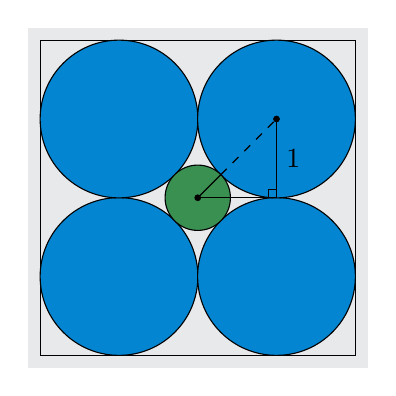
\begin{tikzpicture}[background rectangle/.style={fill=bggray}, show background rectangle]
                \draw[black] (0,0) -- (4,0) -- (4,4) -- (0,4) -- cycle;
                \foreach \x in {1,3}
                    \foreach \y in {1,3}
                        \filldraw[fill=cerulean] (\x,\y) circle (28.5pt);
                \filldraw[fill=strings] (2,2) circle (11.803pt);
                \foreach \x in {2,3}
                    \filldraw[fill=black] (\x,\x) circle (1pt);
                \draw[black] (2,2) -- (3,2) --node[right]{$1$} (3,3);
                \draw[black] (2.9,2) -- (2.9,2.1) -- (3,2.1);
                \draw[black] (2,2) -- (2+0.4142/1.4142, 2+0.4142/1.4142);
                \draw[black, dashed] (2+0.4142/1.4142, 2+0.4142/1.4142) -- (3,3);
            \end{tikzpicture}
        \end{center}
        \caption{Filling 2D square with corner circles and center circle}
    \end{wrapfigure}

    In $\mathbb R^2$, say that we consider the five depicted circles within a $4\times 4$ square. The four ``corner'' circles are tangent to (two) edges of the square and are tangent to each other, with each having radius 1. The ``center'' circle shares its center with the square and is tangent to all four of the corner circles.

    The radius of the center circle is $\sqrt{2} - 1$. Hence, it is smaller than each of the corner circles (as is visibly apparent).

    Generalize this construction to a $4\times 4\times \ldots \times 4$ (hyper)cube in $\mathbb R^d$. In general, there are $2^d$ corner spheres, each having radius 1, and there is one center sphere, with the same center as the hypercube and which is tangent to all of the corner spheres.
\end{frame}

%%%%
\begin{frame}
    \frametitle{Another example of high dimensional weirdness}
    As a consequence of the distance formula in $\mathbb R^d$, the radius of the center sphere is necessarily $\sqrt{d} - 1$. Note the consequences: 
    \begin{itemize}
        \item When $d=4$, then the center sphere is the same size as the corner spheres, since $\sqrt{4}-1 = 1$.
        \item The center sphere is larger than the corner spheres when $d\ge 5$, and once $d = 9$ we have that the radius of the center sphere is $2$. So, that center sphere intersects the boundary of the cube.
        \item For $d\ge 10$, the center sphere contains points that are \textit{outside of} the hypercube. (Despite still being tangent to all $2^d$ corner spheres, which ``surround'' it and are \textit{entirely contained} within the hypercube. Orthogonal projection to any pair of coordinates still looks exactly like the $d=2$ case.)
    \end{itemize}
\end{frame}

\section{Clustering}

\begin{frame}
    \frametitle{What is clustering?}
    Intuitively, want to group together data points into subsets, i.e., \textit{clusters}, so that \textit{similar} points are in the same cluster and dissimilar points are in different clusters. These data do not have labels. 
    
    \begin{itemize}
        \item Presuming the numerical coordinates of the data have meaning, ``similar'' points could be those that are sufficiently close.
    \end{itemize}
    
    \textbf{Goal:} Given sample data $\mathcal S=\{\x_i\}_{i=1}^n$, want to determine clusters $C_1,C_2,\ldots,C_k$ (for some $k$), so that $C_1\cup C_2\cup \ldots\cup C_K= \mathcal S$ and $C_i\cap C_j = \emptyset$ when $i\ne j$.
    \vfill 

    \textit{An inherent difficulty}: the clustering problem is ill-defined. 
    \begin{itemize}
        \item For example, you might have a sequence of data points $\x_1,\ldots,\x_m$ such that $\x_i$ and $\x_{i+1}$ are similar (close enough to be called similar) for each $1\le i\le m-1$, however $\x_1$ and $\x_m$ might be very dissimilar. While $\x_i$ and $x_{i+1}$ should be in the same cluster, this causes the problem of putting $\x_1$ and $\x_m$ ending up in the same cluster.
    \end{itemize}
\end{frame}

\begin{frame}
    \frametitle{Applications of clustering}
    Despite its ill-defined nature, clustering is needed (sometimes in an initial processing step) for many data analysis tasks. 

    Some examples include:
    \begin{itemize}
        \item Market segmentation: clustering expected customers based on characteristics, either for targeted marketing or to inform product design.
        \item Gene expression clustering: computational biologists will cluster genes based on how their expression in different experiments.
        \item Astronomical data analysis: clustering stars or galaxies based on their proximity.
        \item Social network analysis: for example, identifying ``communities'' (clusters of users) based on interactions on social media.
    \end{itemize}
\end{frame}

%%%%
\begin{frame}
    \frametitle{$k$-means}
    Let $\mathcal S=\{\x_i\}_{i=1}^n$, with each $\x_i\in\mathbb R^d$ for some dimension $d$.

    \begin{itemize}
        \item The $k$-means algorithm is a common approach for clustering $\mathcal S$. 
        \item You choose $k$, and your goal is to find $k$ clusters, $C_1, C_2,\ldots, C_k$ so that $\mathcal S=C_1\cup\ldots C_k$, where we want the sum $\sum_{j=1}^k\sum_{\x_i\in C_j} |\x_i - \mu_{j}|^2$ to be minimized. 
        \item Here, $\mu_j$ is the centroid of $C_j$, meaning that $\mu_j$ is the point in $\mathbb R^d$ that minimizes, over $\mu\in\mathbb R^d$, the sum $\sum_{\x\in C_j}|\x - \mu|^2$.
        \begin{itemize}
            \item Note that, in fact, $\mu_j = \frac{1}{|C_j|}\sum_{\x \in C_j}\x$.
        \end{itemize}
    \end{itemize}

    \centering
    \includegraphics[height=0.35\textheight]{../../Images/kmeans_0.png}
\end{frame}

%%%%
\begin{frame}
    \frametitle{$k$-means Procedure}
    
    The procedure to carry out $k$-means clustering is the following. First, randomly initialize $k$ centroids. Then: 
    \begin{enumerate}
        \item For each $i=1,2,\ldots,n$, determine $1\le j(i)\le k$, which is the index such that $\mu_{j(i)}$ is the closest centroid to $\x_i$. A point $\x_i$ is in $C_j$ when $j=j(i)$.
        \item Update $\mu_1,\mu_2,\ldots,\mu_k$ so that, for $1\le j\le k$, the vector $\mu_j$ is the centroid of the points in $C_j$.
        \item Iterate steps 1 and 2 until there is no $\x_i$ that ``changes its cluster'', i.e., until the assignment $i\mapsto j(i)$ that is made in 1 is the same as it was in the previous iteration.
    \end{enumerate}

    At each iteration, if some point has changed the cluster it is in, then the value of $\sum_{j=1}^k\sum_{\x_i\in C_j} |\x_i - \mu_{j}|^2 = \sum_{i=1}^n|\x_i - \mu_{j(i)}|^2$ decreases. Hence, the algorithm terminates because, as there are finitely many points in $\mathcal S$, there are only a finite number of possibilities for the list $\mu_1, \mu_2, \ldots, \mu_k$.
\end{frame}

%%%%
\begin{frame}
    \frametitle{Visual of $k$-means in $\mathbb R^2$}
    
    \begin{wrapfigure}{r}{0.3\textwidth}
        \begin{center}
            \includegraphics[width=0.25\textwidth]{../../Images/kmeans_0.png}
        \end{center}
        \caption{Initial centroids}
    \end{wrapfigure}

    We show a visualization of the procedure for $k$-means on data in $\mathbb R^2$, with $k=2$.
    \vspace*{12pt}

    Initially, we choose two arbitrary centroids. These are drawn in black.

    Then, the first step is to go through all of our data (drawn in ) and determine which of the two centroids is closest to each point. This assigns each point to one of the two clusters.

\vfill
\end{frame}

%%%%
\begin{frame}
    \frametitle{Visual of $k$-means in $\mathbb R^2$}
    
    \begin{wrapfigure}{r}{0.3\textwidth}
        \begin{center}
            \includegraphics[width=0.25\textwidth]{../../Images/kmeans_1.png}
        \end{center}
        \caption{Assigned clusters}
    \end{wrapfigure}

    We show a visualization of the procedure for $k$-means on data in $\mathbb R^2$, with $k=2$.
    \vspace*{12pt}

    Here, the two clusters are shown. 
    
    The points in one are drawn in light blue and the points in the other are drawn in red.  

    The centroid of each cluster is displayed, outlined in the color of its cluster. The next step is to recompute the centroids.

\vfill
\end{frame}

%%%%
\begin{frame}
    \frametitle{Visual of $k$-means in $\mathbb R^2$}
    
    \begin{wrapfigure}{r}{0.3\textwidth}
        \begin{center}
            \includegraphics[width=0.25\textwidth]{../../Images/kmeans_2.png}
        \end{center}
        \caption{Updated clusters}
    \end{wrapfigure}

    We show a visualization of the procedure for $k$-means on data in $\mathbb R^2$, with $k=2$.
    \vspace*{12pt}

    The two newly computed centroids are shown. 
    
    In addition, we reassign points based on the (new) centroid that is closest. 

    We notice that 4 of points have been removed from the blue cluster into the red cluster; also, 3 points have been removed from red cluster into the blue.

\vfill
\end{frame}

%%%%
\begin{frame}
    \frametitle{Visual of $k$-means in $\mathbb R^2$}
    
    \begin{wrapfigure}{r}{0.3\textwidth}
        \begin{center}
            \includegraphics[width=0.25\textwidth]{../../Images/kmeans_3.png}
        \end{center}
        \caption{Updated clusters}
    \end{wrapfigure}

    We show a visualization of the procedure for $k$-means on data in $\mathbb R^2$, with $k=2$.
    \vspace*{12pt}

    Again, we compute new centroids and reassign points based on the centroid that is closest. 
    
    In this step, there is 1 point that was previously in the blue cluster which changes into red. And 4 points that were in the red cluster have been moved into the blue cluster.

\vfill
\end{frame}

%%%%
\begin{frame}
    \frametitle{Visual of $k$-means in $\mathbb R^2$}
    
    \begin{wrapfigure}{r}{0.3\textwidth}
        \begin{center}
            \includegraphics[width=0.25\textwidth]{../../Images/kmeans_4.png}
        \end{center}
        \caption{Updated centroids}
    \end{wrapfigure}

    We show a visualization of the procedure for $k$-means on data in $\mathbb R^2$, with $k=2$.
    \vspace*{12pt}

    We compute new centroids again. 
    
    This time there is no change in the way that points are assigned to clusters when finding the closest centroid. 
    
    Since there is no change to the clustering assignment, the procedure terminates with these centroids.

\vfill
\end{frame}

%%%%
\begin{frame}
    \frametitle{$k$-means depends on Initial Centroids}
    
    \begin{figure}
        \begin{center}
            \includegraphics[height=0.5\textheight]{../../Images/kmeans_balldata0.png}
        \end{center}
        \caption{A data set to cluster}
    \end{figure}
\phantom{With initial centroids of $(0,0.5)$ and $(0, 0.25)$}
\vfill
\end{frame}

%%%%
\begin{frame}
    \frametitle{$k$-means depends on Initial Centroids}
    
    \begin{figure}
        \begin{center}
            \includegraphics[height=0.5\textheight]{../../Images/kmeans_balldata1.png}
        \end{center}
        \caption{A data set to cluster}
    \end{figure}
With initial centroids of $(0,0.5)$ and $(0, 0.25)$.
\vfill
\end{frame}

%%%%
\begin{frame}
    \frametitle{$k$-means depends on Initial Centroids}
    
    \begin{figure}
        \begin{center}
            \includegraphics[height=0.5\textheight]{../../Images/kmeans_balldata2.png}
        \end{center}
        \caption{A data set to cluster}
    \end{figure}
With initial centroids of $(0,0.26)$ and $(0, 0.1)$.
\vfill
\end{frame}

\begin{frame}
    \frametitle{Density-Based Spatial Clustering for Applications with Noise}
    DBSCAN clustering does not require choosing a number of clusters at the start. 

    \begin{itemize}
        \item Near a given point in $\mathcal S$, whether it gets included in a nearby cluster is based on the \textit{density} of points (in $\mathcal S$) near that given point. 
        \item The procedure builds a directed graph (network of vertices and edges); vertices are points in $\mathcal S$; which edges are included is based on a choice of parameters, and takes into account the nearby density of points. 
        \item Connectedness through edges of the graph determines when points are in the same cluster.
    \end{itemize}
    An example of a graph built in the DBSCAN procedure is drawn below. Points are colored according to their cluster.

    \centering
    \includegraphics[height=0.35\textheight]{../../Images/dbscan_graph.png}
\end{frame}

\end{document}